\documentclass[12pt]{article}
\usepackage{../preamble3}
%\pagenumbering{gobble}
\title{MathCounts Competition Practice III, December 2020 \\ Sprint Round}
\author{Patrick \& James Toche}
\date{Revised:~\today}

\begin{document}
\maketitle
\begin{minipage}{\textwidth}
\begin{abstract}\setlength{\parindent}{0pt}%
Notes on Sprint Round of MathCounts Competition Practice III, January 2021. 
Questions are from MathCounts Foundation (\url{https://www.mathcounts.org/}). Copyright restrictions may apply. Written for personal use. 
Please report typos and errors over at \url{https://github.com/ptoche/Math/tree/master/mathcounts}. 
\end{abstract}
\end{minipage}

\thispagestyle{empty}
\clearpage
\addtocounter{page}{-1}

\section*{Sprint Round}


%%%%%%%%%%%%%%%%%%%%%%%%%%%%%%%%%%%%%%%%%%%%%%%%%%%%%%%%%%%%%%%%%%%%%%%%
\subsection*{1.}
How many integers between $500$ and $1000$ contain both the digits $3$ and $4$?

\nopagebreak

\fbox{\phantom{ANSWER}}~integers

\begin{answer}
\begin{tikzpicture}\node[textbox]{%
    \begin{minipagex}{\dimexpr\textwidth-20pt}
        Only two integers, $534$ and $543$, satisfy the criterion between $500$ and $599$. Likewise $634$, $643$ and $734$, $743$ and $834$, $843$ and $934$, $943$. So there are $5 \times 2 = 10$ integers. 
        \begin{empheq}[box={\mathbox[colback=white]}]{equation*}
            10 ~\text{integers}
        \end{empheq}
        
        Note that if the range had been, say, between $300$ and $400$, the calculation would have been different. In this case, valid integers are $34n$, for any $n\in[0,9]$ (ten integers) and $3n4$, for any $n\in[0,9]$ (ten integers). 
    \end{minipagex}
    };
\end{tikzpicture}%
\end{answer}
%%%%%%%%%%%%%%%%%%%%%%%%%%%%%%%%%%%%%%%%%%%%%%%%%%%%%%%%%%%%%%%%%%%%%%%%


%%%%%%%%%%%%%%%%%%%%%%%%%%%%%%%%%%%%%%%%%%%%%%%%%%%%%%%%%%%%%%%%%%%%%%%%
\subsection*{2.}
Tom rides the bus part of the way to school and then he walks the rest of the way. He walks five minutes longer than he rides. The whole trip takes $27$ minutes. For how many minutes does he walk?

\nopagebreak

\fbox{\phantom{ANSWER}}~minutes

\begin{answer}
\begin{tikzpicture}\node[textbox]{%
    \begin{minipagex}{\dimexpr\textwidth-20pt}
        Let $t_1$ denote the time spent riding the bus and $t_2$ the time spent walking. The text suggests the following system (of $2$ equations and $2$ unknown):
        \begin{align*}
        t_2 - t_1 & = 5\\
        t_1 + t_2 & = 27
        \end{align*}
        Adding both equations yields:
        \begin{align*}
        2t_2 & = 5+27\\
        \Rightarrow t_2 & = 16
        \end{align*}
        \begin{empheq}[box={\mathbox[colback=white]}]{equation*}
            16 ~\text{minutes}
        \end{empheq}
    \end{minipagex}
    };
\end{tikzpicture}%
\end{answer}
%%%%%%%%%%%%%%%%%%%%%%%%%%%%%%%%%%%%%%%%%%%%%%%%%%%%%%%%%%%%%%%%%%%%%%%%


%%%%%%%%%%%%%%%%%%%%%%%%%%%%%%%%%%%%%%%%%%%%%%%%%%%%%%%%%%%%%%%%%%%%%%%%
\subsection*{3.}
Liberty Middle School's enrollment increased to $660$ students. This is an increase of $10\%$ over last year's enrollment. What was last year's enrollment?

\nopagebreak

\fbox{\phantom{ANSWER}}~students

\begin{answer}
\begin{tikzpicture}\node[textbox]{%
    \begin{minipagex}{\dimexpr\textwidth-20pt}
        Let $e$ denote last year's enrollment. An increase of $10\%$ is $1.1e$. Thus,
        \begin{align*}
        1.1e = 660 \Rightarrow e = \frac{6,600}{11}= \frac{6\times 11 \times 100}{11} = 600
        \end{align*}
        Last year's enrollment was:
        \begin{empheq}[box={\mathbox[colback=white]}]{equation*}
            600 ~\text{students}
        \end{empheq}
    \end{minipagex}
    };
\end{tikzpicture}%
\end{answer}
%%%%%%%%%%%%%%%%%%%%%%%%%%%%%%%%%%%%%%%%%%%%%%%%%%%%%%%%%%%%%%%%%%%%%%%%


%%%%%%%%%%%%%%%%%%%%%%%%%%%%%%%%%%%%%%%%%%%%%%%%%%%%%%%%%%%%%%%%%%%%%%%%
\subsection*{4.}
The distance from the earth to the sun is $93,000,000$ miles, and light travels at $186,000$ miles per second. How many seconds does light from the sun take to reach the earth?

\nopagebreak

\fbox{\phantom{ANSWER}}~seconds

\begin{answer}
\begin{tikzpicture}\node[textbox]{%
    \begin{minipagex}{\dimexpr\textwidth-20pt}
        The time it takes is given by $t=d/v$, where $t$ is time (seconds), $d$ is distance (miles) and $v$ is velocity (miles per second). To see this quickly, note that velocity $v$ is measured in units of distance per time (miles per second), so that its inverse is in units of time per distance (seconds per mile): keeping track of units shows that $d/v$ is measured in units of time (seconds).  
        \begin{align*}
        \frac{d}{v} 
        = \frac{93,000,000}{186,000} 
          = \frac{93}{186} 10^3
          = \frac{3 \times 31}{3 \times 62} 10^3
          = \frac{1000}{2}
          = 500
        \end{align*}
        Light takes:
        \begin{empheq}[box={\mathbox[colback=white]}]{equation*}
            500 ~\text{seconds}
        \end{empheq}
    \end{minipagex}
    };
\end{tikzpicture}%
\end{answer}
%%%%%%%%%%%%%%%%%%%%%%%%%%%%%%%%%%%%%%%%%%%%%%%%%%%%%%%%%%%%%%%%%%%%%%%%


%%%%%%%%%%%%%%%%%%%%%%%%%%%%%%%%%%%%%%%%%%%%%%%%%%%%%%%%%%%%%%%%%%%%%%%%
\subsection*{5.}
Each of four test scores in Connie's class is to be weighted equally. On the first three tests Connie scored $80\%$, $90\%$ and $95\%$. What percent must she score on her fourth test to have an overall average of exactly $90\%$?

\nopagebreak

\fbox{\phantom{ANSWER}}~\%

\begin{answer}
\begin{tikzpicture}\node[textbox]{%
    \begin{minipagex}{\dimexpr\textwidth-20pt}
        Let $x$ denote the unknown grade. The average is:
        \begin{align*}
        \frac{80 + 90 + 95 + x}{4} = 90
        \end{align*}
        Solving for $x$ yields
        \begin{align*}
        x = 4 \times 90 - 265 = 95
        \end{align*}
        The score on her fourth test is:
        \begin{empheq}[box={\mathbox[colback=white]}]{equation*}
            95\%
        \end{empheq}
    \end{minipagex}
    };
\end{tikzpicture}%
\end{answer}
%%%%%%%%%%%%%%%%%%%%%%%%%%%%%%%%%%%%%%%%%%%%%%%%%%%%%%%%%%%%%%%%%%%%%%%%


%%%%%%%%%%%%%%%%%%%%%%%%%%%%%%%%%%%%%%%%%%%%%%%%%%%%%%%%%%%%%%%%%%%%%%%%
\subsection*{6.}
Haley has enlarged a $3$-inch by $5$-inch picture so that both the length and width are tripled. The area of the enlarged photo is how many times the area of the original photo? 

\nopagebreak

\fbox{\phantom{ANSWER}}~times

\begin{answer}
\begin{tikzpicture}\node[textbox]{%
    \begin{minipagex}{\dimexpr\textwidth-20pt}
        The original area is $3 \times 5$. The enlarged area is $(3 \times 3) \times (3 \times 5)$. The ratio is therefore
        \begin{align*}
        \frac{(3 \times 3) \times (3 \times 5)}{3 \times 5}
        = 3^{2}
        \end{align*}
        \begin{empheq}[box={\mathbox[colback=white]}]{equation*}
            9 ~\text{times}
        \end{empheq}
        This is a general result: scaling up the lengths of a $2$-d figure by a factor $m$ yields to an increase in area of $m^2$. For a $3$-d figure, the increase in volume would be proportional to $m^3$. 
    \end{minipagex}
    };
\end{tikzpicture}%
\end{answer}
%%%%%%%%%%%%%%%%%%%%%%%%%%%%%%%%%%%%%%%%%%%%%%%%%%%%%%%%%%%%%%%%%%%%%%%%


%%%%%%%%%%%%%%%%%%%%%%%%%%%%%%%%%%%%%%%%%%%%%%%%%%%%%%%%%%%%%%%%%%%%%%%%
\subsection*{7.}
What is the least positive integer divisible by each of $1$, $3$, $5$, and $7$?

\nopagebreak

\fbox{\phantom{ANSWER}}

\begin{answer}
\begin{tikzpicture}\node[textbox]{%
    \begin{minipagex}{\dimexpr\textwidth-20pt}
        The least common multiple is
        \begin{align*}
        3 \times 5 \times 7 = 105
        \end{align*}
        \begin{empheq}[box={\mathbox[colback=white]}]{equation*}
            105
        \end{empheq}
    \end{minipagex}
    };
\end{tikzpicture}%
\end{answer}
%%%%%%%%%%%%%%%%%%%%%%%%%%%%%%%%%%%%%%%%%%%%%%%%%%%%%%%%%%%%%%%%%%%%%%%%


%%%%%%%%%%%%%%%%%%%%%%%%%%%%%%%%%%%%%%%%%%%%%%%%%%%%%%%%%%%%%%%%%%%%%%%%
\subsection*{8.}
If $m\Diamond n = (m^2-n)\div n$ for all real numbers $m$ and $n$, where $n\neq0$, what is the value of $6\Diamond3$?

\nopagebreak

\fbox{\phantom{ANSWER}}

\begin{answer}
\begin{tikzpicture}\node[textbox]{%
    \begin{minipagex}{\dimexpr\textwidth-20pt}
        Applying the rule yields
        \begin{align*}
        6\Diamond 3 = (6^2-3) \div 3
        = 33 \div 3
        = 11
        \end{align*}
        \begin{empheq}[box={\mathbox[colback=white]}]{equation*}
            11
        \end{empheq}
    \end{minipagex}
    };
\end{tikzpicture}%
\end{answer}
%%%%%%%%%%%%%%%%%%%%%%%%%%%%%%%%%%%%%%%%%%%%%%%%%%%%%%%%%%%%%%%%%%%%%%%%


%%%%%%%%%%%%%%%%%%%%%%%%%%%%%%%%%%%%%%%%%%%%%%%%%%%%%%%%%%%%%%%%%%%%%%%%
\subsection*{9.}
New York and Denver are in different time zones. When it is noon in New York, it is $10:00a.m.$ in Denver. At $2:00p.m.$ in New York, a train departs, and it arrives in Denver $45$ hours later. What time is it in Denver when the train arrives?

\nopagebreak

\fbox{\phantom{ANSWER}}~a.m.

\begin{answer}
\begin{tikzpicture}\node[textbox]{%
    \begin{minipagex}{\dimexpr\textwidth-20pt}
        The clock resets every $24$ hours. The journey lasts $45$ hours, where $45 = (2\times24)-3$, which we can use for a quick calculation. The train leaves NY at $2p.m.$, so it arrives at $(2-3)p.m.$, which is $11a.m.$ NY time, or $9a.m.$ Denver time.
        \begin{empheq}[box={\mathbox[colback=white]}]{equation*}
            9:00~a.m.
        \end{empheq}
    \end{minipagex}
    };
\end{tikzpicture}%
\end{answer}
%%%%%%%%%%%%%%%%%%%%%%%%%%%%%%%%%%%%%%%%%%%%%%%%%%%%%%%%%%%%%%%%%%%%%%%%


%%%%%%%%%%%%%%%%%%%%%%%%%%%%%%%%%%%%%%%%%%%%%%%%%%%%%%%%%%%%%%%%%%%%%%%%
\subsection*{10.}
A month ago, the ratio of nurses to doctors on a hospital staff was $3{:}5$. Since that time, two additional nurses joined the staff, no nurses left and the number of doctors remained the same. The ratio of nurses to doctors on the hospital staff is now $4{:}5$. How many nurses are \textbf{now} on the staff?

\nopagebreak

\fbox{\phantom{ANSWER}}~nurses

\begin{answer}
\begin{tikzpicture}\node[textbox]{%
    \begin{minipagex}{\dimexpr\textwidth-20pt}
        Let $n$ denote the number of nurses and $d$ the number of doctors one month ago. The verbal statement yields a linear system in $n$ and $d$:
        \begin{align*}
        \frac{n}{d} & = \frac{3}{5}\\
        \frac{n+2}{d} & = \frac{4}{5}\\
        \end{align*}
        Or equivalently:
        \begin{align*}
        3d - 5n & = 0 \\
        4d - 5n & = 10 
        \end{align*}
        Subtracting the first equation from the second gives $d=10$, from which $n=6$ follows. And so $n+2=8$. 
        \begin{empheq}[box={\mathbox[colback=white]}]{equation*}
            8~\text{nurses}
        \end{empheq}
    \end{minipagex}
    };
\end{tikzpicture}%
\end{answer}
%%%%%%%%%%%%%%%%%%%%%%%%%%%%%%%%%%%%%%%%%%%%%%%%%%%%%%%%%%%%%%%%%%%%%%%%


%%%%%%%%%%%%%%%%%%%%%%%%%%%%%%%%%%%%%%%%%%%%%%%%%%%%%%%%%%%%%%%%%%%%%%%%
\subsection*{11.}
A sequence is formed by multiplying each term by $3$ and then adding $3$ to get the next term. If the third term is $39$, what is the value of the first term? 

\nopagebreak

\fbox{\phantom{ANSWER}}

\begin{answer}
\begin{tikzpicture}\node[textbox]{%
    \begin{minipagex}{\dimexpr\textwidth-20pt}
        To go backwards from the third to the first term, we apply the reverse steps twice. We first subtract $3$, then divide by $3$, starting from $39$. 
        \begin{align*}
        (39 - 3) /3 & = 12\\
        (12 - 3)/3  & = 3
        \end{align*}
        The first term is:
        \begin{empheq}[box={\mathbox[colback=white]}]{equation*}
            3
        \end{empheq}
    \end{minipagex}
    };
\end{tikzpicture}%
\end{answer}
%%%%%%%%%%%%%%%%%%%%%%%%%%%%%%%%%%%%%%%%%%%%%%%%%%%%%%%%%%%%%%%%%%%%%%%%


%%%%%%%%%%%%%%%%%%%%%%%%%%%%%%%%%%%%%%%%%%%%%%%%%%%%%%%%%%%%%%%%%%%%%%%%
\subsection*{12.}
Bill and Jill both exercise on Monday, January 1. Bill exercises every $5$th day, and Jill exercises every $4$th day. What is the next date on which Bill and Jill both exercise?

\nopagebreak

\fbox{\phantom{ANSWER}}\fbox{\phantom{ANSWER}}

\begin{answer}
\begin{tikzpicture}\node[textbox]{%
    \begin{minipagex}{\dimexpr\textwidth-20pt}
        The least common multiple is $5 \times 4 = 20$. They exercise on the same day every $20$ days. 
        \begin{empheq}[box={\mathbox[colback=white]}]{equation*}
            01 (January), 21st
        \end{empheq}
    \end{minipagex}
    };
\end{tikzpicture}%
\end{answer}
%%%%%%%%%%%%%%%%%%%%%%%%%%%%%%%%%%%%%%%%%%%%%%%%%%%%%%%%%%%%%%%%%%%%%%%%


%%%%%%%%%%%%%%%%%%%%%%%%%%%%%%%%%%%%%%%%%%%%%%%%%%%%%%%%%%%%%%%%%%%%%%%%
\subsection*{13.}
Consider the square with vertices at $(3,3)$, $(-3,3)$, $(-3,-3)$ and $(3,-3)$. How many points with integer coordinates lie strictly in the interior of this square?

\nopagebreak

\fbox{\phantom{ANSWER}}~points

\begin{answer}
\begin{tikzpicture}\node[textbox]{%
    \begin{minipagex}{\dimexpr\textwidth-20pt}
        Because the figure is a square, we can count the points along one edge and square that number. The horizontal length between $-3$ and $3$ contains points at $-2$, $-1$, $0$, $+1$, $+2$, or five points:
        \begin{align*}
        5^2 = 25
        \end{align*}
        \begin{empheq}[box={\mathbox[colback=white]}]{equation*}
            25 ~\text{points}
        \end{empheq}
    \end{minipagex}
    };
\end{tikzpicture}%
\end{answer}
%%%%%%%%%%%%%%%%%%%%%%%%%%%%%%%%%%%%%%%%%%%%%%%%%%%%%%%%%%%%%%%%%%%%%%%%


%%%%%%%%%%%%%%%%%%%%%%%%%%%%%%%%%%%%%%%%%%%%%%%%%%%%%%%%%%%%%%%%%%%%%%%%
\subsection*{14.}
A bracelet is made by stringing together four beads. Each bead is either red or green. How many different color patterns are possible for the bracelet, where the patterns are considered the same if rotating one will produce the other, as shown here? 

\nopagebreak

\fbox{\phantom{ANSWER}}~patterns

\begin{minipagex}[b]{\linewidth}
\centering
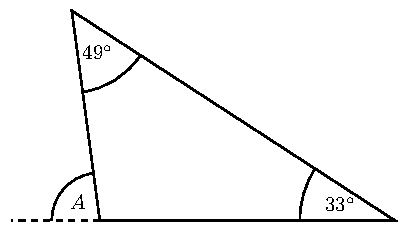
\includegraphics[height=2.5cm]{sprint-14-figure}
\end{minipagex}

\begin{answer}
\begin{tikzpicture}\node[textbox]{%
    \begin{minipagex}{\dimexpr\textwidth-20pt}
        We are not told how many beads of each color to string. ``Each bead is either red or green'' means that the beads must be either red or green, including possibly all red or all green. There are therefore $4$ possibilities:
        \begin{enumerate}
        \item Colors: $\{GGGG\}$. Patterns: $[GGGG]$. Count: $1$
        \item Colors: $\{RGGG\}$. Patterns: $[RGGG]$. Count: $1$
        \item Colors: $\{RRGG\}$. Patterns: $[RRGG, RGRG]$. Count: $2$
        \item Colors: $\{RRRG\}$. Patterns: $[RRRG]$. Count: $1$
        \item Colors: $\{RRRR\}$. Patterns: $[RRRR]$. Count: $1$
        \end{enumerate}
        Note: $RGGR$ is a repeat of $RRGG$ by rotation. 
        Total: $1+1+2+1+1=6$
        \begin{empheq}[box={\mathbox[colback=white]}]{equation*}
            6 ~\text{patterns}
        \end{empheq}
    \end{minipagex}
    };
\end{tikzpicture}%
\end{answer}
%%%%%%%%%%%%%%%%%%%%%%%%%%%%%%%%%%%%%%%%%%%%%%%%%%%%%%%%%%%%%%%%%%%%%%%%


%%%%%%%%%%%%%%%%%%%%%%%%%%%%%%%%%%%%%%%%%%%%%%%%%%%%%%%%%%%%%%%%%%%%%%%%
\subsection*{15.}
To create a unique house paint color, Melton mixes together a sample that is $12$ gallons of red, $2.5$ gallons of yellow and $0.5$ gallons of blue paint. He then mixes a main batch of paint using $30$ gallons of yellow paint and enough red and blue paint to maintain the original ratio. How many total gallons of paint did he use to make the main batch of paint?

\nopagebreak

\fbox{\phantom{ANSWER}}~gallons

\begin{answer}
\begin{tikzpicture}\node[textbox]{%
    \begin{minipagex}{\dimexpr\textwidth-20pt}
        The sample mix of red/yellow/blue weighs $(12 + 2.5 + 0.5)$ gallons. The main batch is increased in proportion by the same factor that $2.5$ is increased to $30$, a factor of $12$:
        \begin{align*}
        \frac{30}{2.5} = 12
        \end{align*}
        The main batch therefore weighs: 
        \begin{align*}
        12\times(12 + 2.5 + 0.5) 
          = 12\times12 + 12\times2.5 + 12\times0.5
          = 144 + 30 + 6
          = 180
        \end{align*}
        The total weight is:
        \begin{empheq}[box={\mathbox[colback=white]}]{equation*}
            180~\text{gallons}
        \end{empheq}
    \end{minipagex}
    };
\end{tikzpicture}%
\end{answer}
%%%%%%%%%%%%%%%%%%%%%%%%%%%%%%%%%%%%%%%%%%%%%%%%%%%%%%%%%%%%%%%%%%%%%%%%


%%%%%%%%%%%%%%%%%%%%%%%%%%%%%%%%%%%%%%%%%%%%%%%%%%%%%%%%%%%%%%%%%%%%%%%%
\subsection*{16.}
How many different squares can be formed by using four of the evenly spaced dots shown as vertices of the square?

\nopagebreak

\fbox{\phantom{ANSWER}}~squares

\begin{minipagex}[b]{\linewidth}
\centering

\includegraphics[height=2cm]{sprint-16-figure}
\end{minipagex}

\begin{answer}
\begin{tikzpicture}\node[textbox]{%
    \begin{minipagex}{\dimexpr\textwidth-20pt}
        Let the distance between two adjacent dots be $1$ unit. There are $6$ squares formed by connecting four dots separated by $1$ unit. There are $2$ squares formed by connecting four dots separated by $2$ units. In addition, there are $2$ squares formed by connecting four dots separated by $\sqrt{2}$ units (along a diagonal).
        \begin{align*}
        6 + 2 + 2 = 10
        \end{align*}
        \begin{empheq}[box={\mathbox[colback=white]}]{equation*}
            10~\text{squares}
        \end{empheq}
    \end{minipagex}
    };
\end{tikzpicture}%
\end{answer}
%%%%%%%%%%%%%%%%%%%%%%%%%%%%%%%%%%%%%%%%%%%%%%%%%%%%%%%%%%%%%%%%%%%%%%%%


%%%%%%%%%%%%%%%%%%%%%%%%%%%%%%%%%%%%%%%%%%%%%%%%%%%%%%%%%%%%%%%%%%%%%%%%
\subsection*{17.}
Xinran walks $3$ mi/h uphill, $4$ mi/h on flat land and $5$ mi/h downhill. If he walks one mile uphill, then one mile on flat land and then returns by the same route to his starting point, how many minutes does he walk? 

\nopagebreak

\fbox{\phantom{ANSWER}}~minutes

\begin{answer}
\begin{tikzpicture}\node[textbox]{%
    \begin{minipagex}{\dimexpr\textwidth-20pt}
        At a speed of $3$ mi/h uphill, Xinran walks $1$ mile in $1/3$ of an hour -- or $20$ minutes. At a speed of $4$ mi/h on flat, Xinran walks $1$ mile in $1/4$ of an hour -- or $15$ minutes. At a speed of $5$ mi/h downhill, Xinran walks $1$ mile in $1/5$ of an hour -- or $12$ minutes. Since Xinran backtracks after one mile, he walks a total of two miles on flat. Thus,
        \begin{align*}
        \left(\frac{1}{3} \times 60'\right) + 2 \times \left(\frac{1}{4} \times 60'\right) + \left(\frac{1}{5} \times 60'\right)
        = 20' + 30' + 12'
        = 62'
        \end{align*}
        \begin{empheq}[box={\mathbox[colback=white]}]{equation*}
            62~\text{minutes}
        \end{empheq}
    \end{minipagex}
    };
\end{tikzpicture}%
\end{answer}
%%%%%%%%%%%%%%%%%%%%%%%%%%%%%%%%%%%%%%%%%%%%%%%%%%%%%%%%%%%%%%%%%%%%%%%%


%%%%%%%%%%%%%%%%%%%%%%%%%%%%%%%%%%%%%%%%%%%%%%%%%%%%%%%%%%%%%%%%%%%%%%%%
\subsection*{18.}
Sassy Fashions buys dresses at wholesale and then marks them up for retail sale. They recently sold a dress at $40\%$ discount off their marked-up price. What percent mark-up did they originally apply to the dress if they broke even on the sale? Express your answer to the nearest whole percent. 

\nopagebreak

\fbox{\phantom{ANSWER}}~\%

\begin{answer}
\begin{tikzpicture}\node[textbox]{%
    \begin{minipagex}{\dimexpr\textwidth-20pt}
        Let $m$ denote the markup and $c$ the cost of the dress at wholesale. The store breaks even if they sell the dress at cost. In other words, the discount exactly offsets the markup:
        \begin{align*}
        c & = 0.6 (1+m) c \\
        \Rightarrow 1+m & = \frac{1}{0.6} 
        \Rightarrow m = \frac{10}{6} -1 = \frac{5-3}{3} = \frac{2}{3}
        \end{align*}
        \begin{empheq}[box={\mathbox[colback=white]}]{equation*}
            67~\%
        \end{empheq}
    \end{minipagex}
    };
\end{tikzpicture}%
\end{answer}
%%%%%%%%%%%%%%%%%%%%%%%%%%%%%%%%%%%%%%%%%%%%%%%%%%%%%%%%%%%%%%%%%%%%%%%%


%%%%%%%%%%%%%%%%%%%%%%%%%%%%%%%%%%%%%%%%%%%%%%%%%%%%%%%%%%%%%%%%%%%%%%%%
\subsection*{19.}
For integers $a$, $b$ and $k$, we know that $a>12$, $b<20$ and $a<b$. If $b=7k$, what is the value of $k$? 

\nopagebreak

\fbox{\phantom{ANSWER}}

\begin{answer}
\begin{tikzpicture}\node[textbox]{%
    \begin{minipagex}{\dimexpr\textwidth-20pt}
        $b$ is a multiple of $7$ between $12$ and $20$:
        \begin{align*}
        b = 14 \Rightarrow k = 2
        \end{align*}
        \begin{empheq}[box={\mathbox[colback=white]}]{equation*}
            2
        \end{empheq}
    \end{minipagex}
    };
\end{tikzpicture}%
\end{answer}
%%%%%%%%%%%%%%%%%%%%%%%%%%%%%%%%%%%%%%%%%%%%%%%%%%%%%%%%%%%%%%%%%%%%%%%%


%%%%%%%%%%%%%%%%%%%%%%%%%%%%%%%%%%%%%%%%%%%%%%%%%%%%%%%%%%%%%%%%%%%%%%%%
\subsection*{20.}
If one quart of paint is exactly enough for two coats of paint on a $9$-foot by $10$-foot wall, how many quarts of paint are needed to apply one coat of paint to a $10$-foot by $12$-foot wall? Express your answer as a common fraction.

\nopagebreak

\begin{minipage}[b]{\linewidth}
\fbox{\phantom{ANSWER}}\\
\mbox{---------------}~~quarts\\
\fbox{\phantom{ANSWER}}
\end{minipage}

\begin{answer}
\begin{tikzpicture}\node[textbox]{%
    \begin{minipagex}{\dimexpr\textwidth-20pt}
        Two coats cover $9 \times 10$ square feet, so one coat ($0.5$ quart) covers $45ft^2$. The amount of paint needed to cover $1ft^2$ is therefore $\dfrac{0.5}{45}$. The amount of paint needed to cover $120ft^2$ is:
        \begin{align*}
        120 \times \frac{0.5}{45} = \frac{120}{90} = \frac{4}{3}
        \end{align*}
        \begin{empheq}[box={\mathbox[colback=white]}]{equation*}
            \frac{4}{3}~\text{quarts}
        \end{empheq}
    \end{minipagex}
    };
\end{tikzpicture}%
\end{answer}
%%%%%%%%%%%%%%%%%%%%%%%%%%%%%%%%%%%%%%%%%%%%%%%%%%%%%%%%%%%%%%%%%%%%%%%%


%%%%%%%%%%%%%%%%%%%%%%%%%%%%%%%%%%%%%%%%%%%%%%%%%%%%%%%%%%%%%%%%%%%%%%%%
\subsection*{21.}
A mixture is made with $45$ ounces of a $10\%$ saline solution and $x$ ounces of a $70\%$ saline solution. The resulting mixture is a $25\%$ saline solution. What is the value of $x$? 

\nopagebreak

\fbox{\phantom{ANSWER}}

\begin{answer}
\begin{tikzpicture}\node[textbox]{%
    \begin{minipagex}{\dimexpr\textwidth-20pt}
        $45$ ounces of a $10\%$ solution contains $0.1 \times 45$ ounces of salt, while $x$ ounces of a $70\%$ solution contains $0.7x$ ounces of salt. The resulting mix weighs $45+x$ ounces. Therefore:
        \begin{align*}
        0.1 \times 45 + 0.7 x & = 0.25 \times (45 + x)
        \end{align*}
        Instead of dealing with decimals and risking a silly mistake, multiply through by $100$. 
        \begin{align*}
        10 \times 45 + 70x & = 25 \times 45 + 25x \\
        \Rightarrow
        (70-25) x & = 25 \times 45 - 10 \times 45 \\
        \Rightarrow
        45 x & = 45 (25 - 10)\\
        \Rightarrow
        x & = 25 - 10 = 15
        \end{align*}        \begin{empheq}[box={\mathbox[colback=white]}]{equation*}
            15
        \end{empheq}
    \end{minipagex}
    };
\end{tikzpicture}%
\end{answer}
%%%%%%%%%%%%%%%%%%%%%%%%%%%%%%%%%%%%%%%%%%%%%%%%%%%%%%%%%%%%%%%%%%%%%%%%


%%%%%%%%%%%%%%%%%%%%%%%%%%%%%%%%%%%%%%%%%%%%%%%%%%%%%%%%%%%%%%%%%%%%%%%%
\subsection*{22.}
In the figure, the hexagon with the ``R'' is colored red, and each of the other hexagons will be colored red, yellow or green, so that no two hexagons with a common side are the same color. In how many different ways can the figure be colored?

\nopagebreak

\fbox{\phantom{ANSWER}}~ways

\begin{minipagex}[b]{\linewidth}
\centering
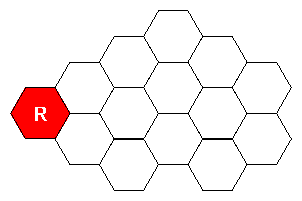
\includegraphics[height=3cm]{sprint-22-figure-1}
\end{minipagex}

\begin{answer}
\begin{tikzpicture}\node[textbox]{%
    \begin{minipagex}{\dimexpr\textwidth-20pt}
        There are $2$ choices at the first node. Beyond that, the choice of colors is unique. The two solutions are:
        \begin{center}
        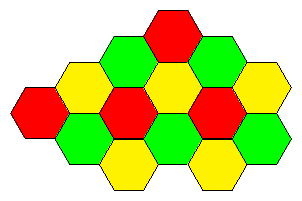
\includegraphics[height=3cm]{sprint-22-figure-2}
        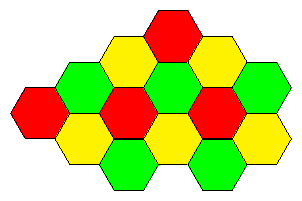
\includegraphics[height=3cm]{sprint-22-figure-3}
        \end{center}
        \begin{empheq}[box={\mathbox[colback=white]}]{equation*}
            2~\text{ways}
        \end{empheq}
    \end{minipagex}
    };
\end{tikzpicture}%
\end{answer}
%%%%%%%%%%%%%%%%%%%%%%%%%%%%%%%%%%%%%%%%%%%%%%%%%%%%%%%%%%%%%%%%%%%%%%%%


%%%%%%%%%%%%%%%%%%%%%%%%%%%%%%%%%%%%%%%%%%%%%%%%%%%%%%%%%%%%%%%%%%%%%%%%
\subsection*{23.}
Five numbered balls, each with a different number from $1$ through $5$, are placed in a bowl. If Josh randomly chooses two balls, with replacement, what is the probability that the two numbers on the selected balls have a product that is even and greater than $10$? Express your answer as a common fraction. 

\nopagebreak

\begin{minipage}[b]{\linewidth}
\fbox{\phantom{ANSWER}}\\
\mbox{---------------}\\
\fbox{\phantom{ANSWER}}
\end{minipage}

\begin{answer}
\begin{tikzpicture}\node[textbox]{%
    \begin{minipagex}{\dimexpr\textwidth-20pt}
        If Josh picks either a $1$ or a $2$, the product cannot exceed $10$ no matter what the other ball is. There are five pairs that work: $(3,4)$, $(4,3)$, $(4,4)$, $(3,4)$, $(4,5)$, $(5,4)$. Since there are $5 \times 5 = 25$ possible pairs, the probability is
        \begin{align*}
        \frac{5}{25} = \frac{1}{5}
        \end{align*}
        \begin{empheq}[box={\mathbox[colback=white]}]{equation*}
            \frac{1}{5} 
        \end{empheq}
    \end{minipagex}
    };
\end{tikzpicture}%
\end{answer}
%%%%%%%%%%%%%%%%%%%%%%%%%%%%%%%%%%%%%%%%%%%%%%%%%%%%%%%%%%%%%%%%%%%%%%%%


%%%%%%%%%%%%%%%%%%%%%%%%%%%%%%%%%%%%%%%%%%%%%%%%%%%%%%%%%%%%%%%%%%%%%%%%
\subsection*{24.}
On Claudia's birthday in $2019$, her age was four times her brother's age on that day. On her birthday in $2020$, her age was three times her brother's age on that day. In what year will Claudia's age, on her birthday, be twice her brother's age on that day?

\nopagebreak

\fbox{\phantom{ANSWER}}

\begin{answer}
\begin{tikzpicture}\node[textbox]{%
    \begin{minipagex}{\dimexpr\textwidth-20pt}
        Let $c$ be Claudia's age, $b$ her brother's age, and $x$ the number of years that will pass. We have
        \begin{align*}
        c & = 4 b\\
        c + 1 & = 3(b+1)\\
        c + x & = 2(b+x)
        \end{align*}
        Solving the system by substitution yields $c=8$, $b=2$, and $x=4$.
        \begin{align*}
        2019 + 4 = 2023
        \end{align*}    
        \begin{empheq}[box={\mathbox[colback=white]}]{equation*}
            2023
        \end{empheq}
    \end{minipagex}
    };
\end{tikzpicture}%
\end{answer}
%%%%%%%%%%%%%%%%%%%%%%%%%%%%%%%%%%%%%%%%%%%%%%%%%%%%%%%%%%%%%%%%%%%%%%%%


%%%%%%%%%%%%%%%%%%%%%%%%%%%%%%%%%%%%%%%%%%%%%%%%%%%%%%%%%%%%%%%%%%%%%%%%
\subsection*{25.}
What is the area of the pentagon shown, with the indicated side lengths in inches? 

\nopagebreak

\fbox{\phantom{ANSWER}}~in$^2$

\begin{minipagex}[b]{\linewidth}
\centering
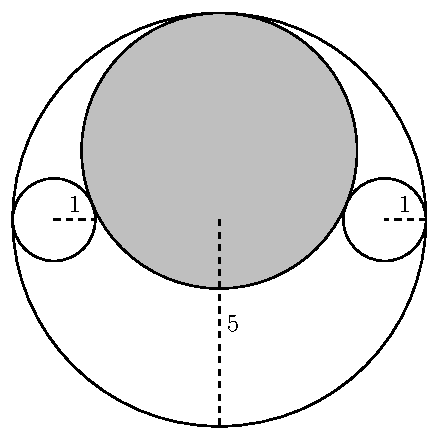
\includegraphics[height=5cm]{sprint-25-figure}
\end{minipagex}

\begin{answer}
\begin{tikzpicture}\node[textbox]{%
    \begin{minipagex}{\dimexpr\textwidth-20pt}
        Breaking down the areas into a rectangle and two triangles yields:
        \begin{align*}
        12 \cdot 8 + 2 \left(\frac{1}{2} \cdot 8 \cdot 6\right)
          = 12 \cdot 8 + 8 \cdot 6
          = 8 (12 + 6)
          = 8 \cdot 18
          = 144 
        \end{align*}
        \begin{empheq}[box={\mathbox[colback=white]}]{equation*}
            144~\text{in}^2
        \end{empheq}
    \end{minipagex}
    };
\end{tikzpicture}%
\end{answer}
%%%%%%%%%%%%%%%%%%%%%%%%%%%%%%%%%%%%%%%%%%%%%%%%%%%%%%%%%%%%%%%%%%%%%%%%


%%%%%%%%%%%%%%%%%%%%%%%%%%%%%%%%%%%%%%%%%%%%%%%%%%%%%%%%%%%%%%%%%%%%%%%%
\subsection*{26.}
A bag contains exactly three red marbles, five yellow marbles and two blue marbles. If three marbles are drawn from the bag without replacement, what is the probability that all three will be the same color? Express your answer as a common fraction.

\nopagebreak

\begin{minipage}[b]{\linewidth}
\fbox{\phantom{ANSWER}}\\
\mbox{---------------}\\
\fbox{\phantom{ANSWER}}
\end{minipage}

\begin{answer}
\begin{tikzpicture}\node[textbox]{%
    \begin{minipagex}{\dimexpr\textwidth-20pt}
        Three marbles of the same color could only be red or yellow. There are $10$ marbles to begin with. The probability of drawing exactly three red marbles is:
        \begin{align*}
        \frac{3}{10} \times \frac{2}{9} \times \frac{1}{8}
        \end{align*}
        The probability of drawing exactly three yellow marbles is:
        \begin{align*}
        \frac{5}{10} \times \frac{4}{9} \times \frac{3}{8}
        \end{align*}
        Adding up the probabilities:
        \begin{align*}
        \frac{3}{10} \times \frac{2}{9} \times \frac{1}{8} +
        \frac{5}{10} \times \frac{4}{9} \times \frac{3}{8} 
          = \frac{3 \times 2 + 5 \times 4 \times 3}{10 \times 9 \times 8} 
          = \frac{66}{720} 
          = \frac{33}{360}
          = \frac{11}{120}
        \end{align*}
        \begin{empheq}[box={\mathbox[colback=white]}]{equation*}
            \frac{11}{120}
        \end{empheq}
    \end{minipagex}
    };
\end{tikzpicture}%
\end{answer}
%%%%%%%%%%%%%%%%%%%%%%%%%%%%%%%%%%%%%%%%%%%%%%%%%%%%%%%%%%%%%%%%%%%%%%%%


%%%%%%%%%%%%%%%%%%%%%%%%%%%%%%%%%%%%%%%%%%%%%%%%%%%%%%%%%%%%%%%%%%%%%%%%
\subsection*{27.}
A peep increased by $25\%$ is a pop. A pop decreased by $40\%$ is a slug, and a slug increased by $100\%$ is a slap. What percent of a peep is a slap? 

\nopagebreak

\fbox{\phantom{ANSWER}}~\%

\begin{answer}
\begin{tikzpicture}\node[textbox]{%
    \begin{minipagex}{\dimexpr\textwidth-20pt}
        The relationships are:
        \begin{align*}
        \text{pop} & = (1+0.25) ~\text{peep} \\
        \text{slug} & = (1-0.4) ~\text{pop} \\
        \text{slap} & = (1+1) ~\text{slug}
        \end{align*}
        The relationship between a peep is a slap is:
        \begin{align*}
        \text{slap} & = (1+1) (1-0.4) (1+0.25) ~\text{peep} \\
             & = 2 \cdot 0.6 \cdot 1.25 ~\text{peep} \\
             & = 1.5 ~\text{peep}
        \end{align*}
        \begin{empheq}[box={\mathbox[colback=white]}]{equation*}
            150~\%
        \end{empheq}
    \end{minipagex}
    };
\end{tikzpicture}%
\end{answer}
%%%%%%%%%%%%%%%%%%%%%%%%%%%%%%%%%%%%%%%%%%%%%%%%%%%%%%%%%%%%%%%%%%%%%%%%


%%%%%%%%%%%%%%%%%%%%%%%%%%%%%%%%%%%%%%%%%%%%%%%%%%%%%%%%%%%%%%%%%%%%%%%%
\subsection*{28.}
If Jonah reverses the two digits of his age, divides the resulting number by three, and then adds $20$, the result is Jonah's age. How old is Jonah? 

\nopagebreak

\fbox{\phantom{ANSWER}}~years old

\begin{answer}
\begin{tikzpicture}\node[textbox]{%
    \begin{minipagex}{\dimexpr\textwidth-20pt}
        Let $x$ and $y$ denote the digits. Jonah's age may be written $10x+y$. The verbal statement yields the equation:
        \begin{align*}
        \frac{10y + x}{3} + 20 = 10x + y
        \end{align*}
        Multiplying through by $3$ and combining terms yields:
        \begin{align*}
        29x = 7y + 60
        \end{align*}
        Based on trial and error (starting with low values of $x$ and matching the last digit of multiples of $7$), we find $x = 4$ and $y = 8$. 
        \begin{empheq}[box={\mathbox[colback=white]}]{equation*}
            48~\text{years old}
        \end{empheq}
    \end{minipagex}
    };
\end{tikzpicture}%
\end{answer}
%%%%%%%%%%%%%%%%%%%%%%%%%%%%%%%%%%%%%%%%%%%%%%%%%%%%%%%%%%%%%%%%%%%%%%%%


%%%%%%%%%%%%%%%%%%%%%%%%%%%%%%%%%%%%%%%%%%%%%%%%%%%%%%%%%%%%%%%%%%%%%%%%
\subsection*{29.}
In the figure shown, the sequence of integers in the row of squares and in each of the two columns of squares form three distinct arithmetic sequences. What is the value of $N$? 

\nopagebreak

\fbox{\phantom{ANSWER}}

\begin{minipagex}[b]{\linewidth}
\centering
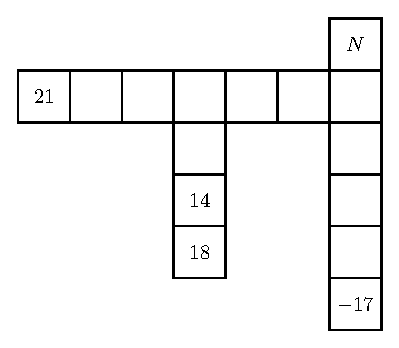
\includegraphics[height=5cm]{sprint-29-figure-1}
\end{minipagex}

\begin{answer}
\begin{tikzpicture}\node[textbox]{%
    \begin{minipagex}{\dimexpr\textwidth-20pt}
        Refer to the figure. Since these are arithmetic sequences, we subtract $4$ from $18$ to get $14$, $10$, $6$. This means we go from $21$ down to $6$ in three steps, i.e. by subtracting $15/3=5$ at each step. Thus going rightwards from $6$ yields $1$, $-4$, and $-9$ (immediately below $N$). This means we go from $-17$ to $-9$ in four steps, i.e. by adding $8/4=2$ at each step. This implies
        \begin{align*}
        N = -9 + 2 = -7
        \end{align*}
        Complete solution: \newline
        \begin{minipagex}[b]{\linewidth}
        \centering
        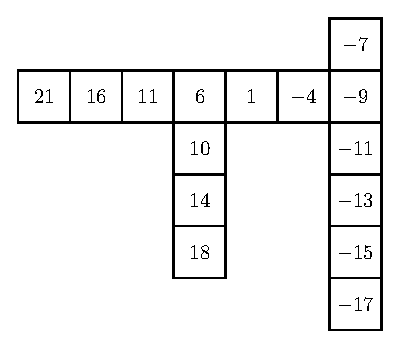
\includegraphics[height=5cm]{sprint-29-figure-2}
        \end{minipagex}
        \begin{empheq}[box={\mathbox[colback=white]}]{equation*}
            -7
        \end{empheq}
    \end{minipagex}
    };
\end{tikzpicture}%
\end{answer}
%%%%%%%%%%%%%%%%%%%%%%%%%%%%%%%%%%%%%%%%%%%%%%%%%%%%%%%%%%%%%%%%%%%%%%%%


%%%%%%%%%%%%%%%%%%%%%%%%%%%%%%%%%%%%%%%%%%%%%%%%%%%%%%%%%%%%%%%%%%%%%%%%
\subsection*{30.}
If $\dfrac{a}{b}=\dfrac{3}{4}$, $\dfrac{b}{c}=\dfrac{8}{9}$, and $\dfrac{c}{d}=\dfrac{2}{3}$, what is the value of $\dfrac{ad}{b^2}$? Express your answer as a common fraction. 

\nopagebreak

\begin{minipage}[b]{\linewidth}
\fbox{\phantom{ANSWER}}\\
\mbox{---------------}\\
\fbox{\phantom{ANSWER}}
\end{minipage}

\begin{answer}
\begin{tikzpicture}\node[textbox]{%
    \begin{minipagex}{\dimexpr\textwidth-20pt}
        \begin{align*}
        \frac{a}{b} & = \frac{3}{4}\\
        \frac{b}{c} & = \frac{8}{9}\\
        \frac{c}{d} & = \frac{2}{3}
        \end{align*}
        By dividing the first equation by the second and third equations, we get
        \begin{align*}
        \frac{a}{b} \times \frac{c}{b} \times \frac{d}{c}
          & = \frac{3}{4} \times \frac{9}{8} \times \frac{3}{2} \\
        \frac{ad}{b^2} & = \frac{3 \times 9 \times 3}{4 \times 8 \times 2} \\
                       & = \frac{81}{64}
        \end{align*}
        \begin{empheq}[box={\mathbox[colback=white]}]{equation*}
            \frac{81}{64}
        \end{empheq}
    \end{minipagex}
    };
\end{tikzpicture}%
\end{answer}
%%%%%%%%%%%%%%%%%%%%%%%%%%%%%%%%%%%%%%%%%%%%%%%%%%%%%%%%%%%%%%%%%%%%%%%%


\end{document}